\section*{Consulta 4: Países que han ganado más medallas por disciplina}

\subsection*{Descripción}

\textbf{SQL}

\begin{verbatim}
SELECT 
    p.NombrePais,
    d.NombreDisciplina,
    COUNT(m.TipoMedalla) AS CantidadMedallas
FROM 
    Medalla m
JOIN 
    Atleta a ON m.IDAtleta = a.IDAtleta
JOIN 
    Disciplina d ON m.IDDisciplina = d.IDDisciplina
JOIN 
    Pais p ON a.NombrePais = p.NombrePais
GROUP BY 
    p.NombrePais, d.NombreDisciplina
ORDER BY 
    CantidadMedallas DESC;
\end{verbatim}

\begin{center}
    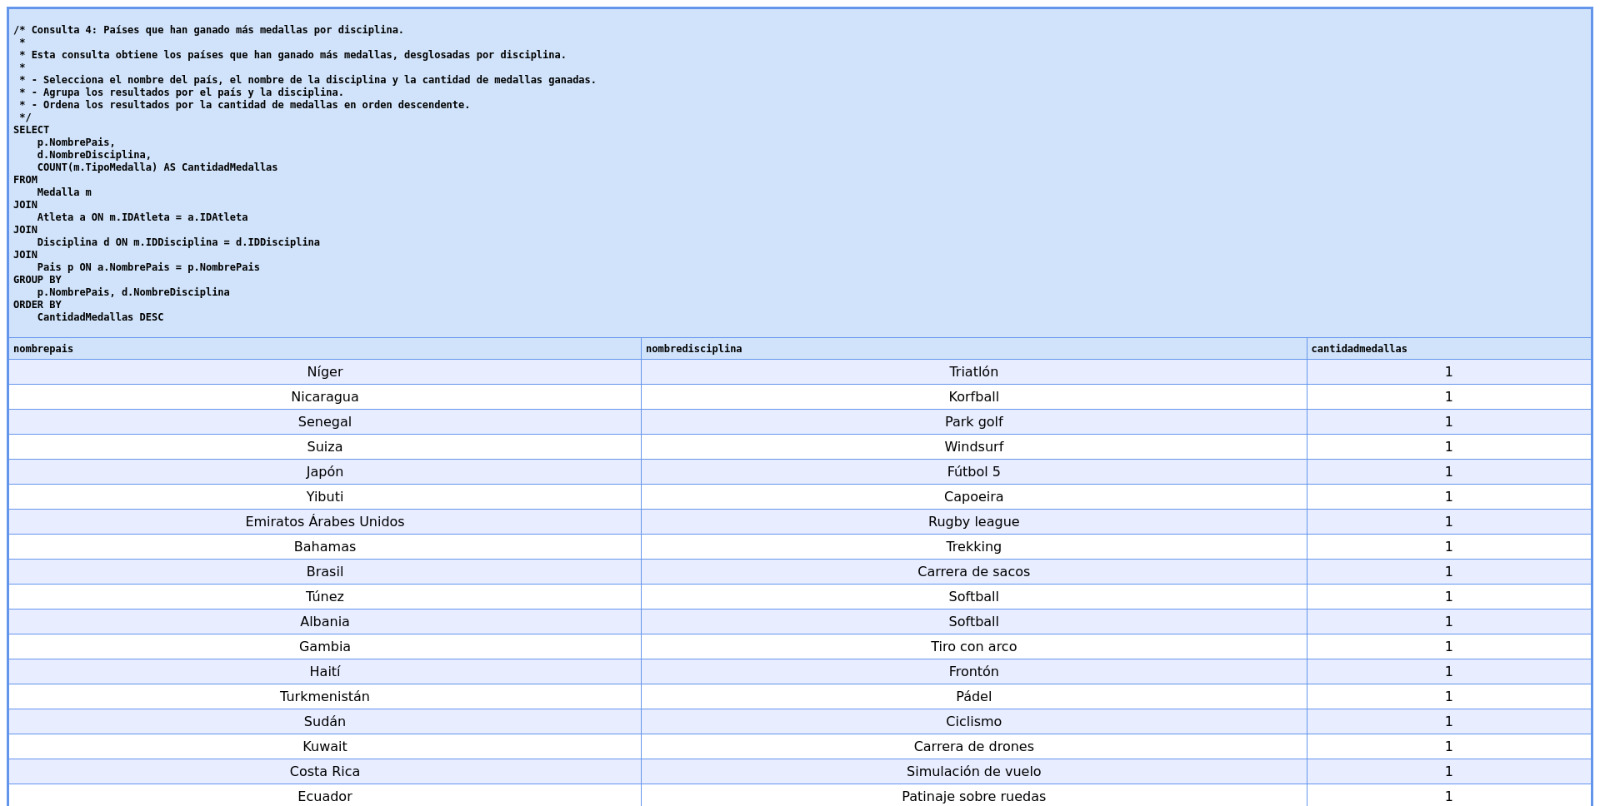
\includegraphics[width=16.5cm]{../resources/Chapters/Consultas/Imagenes/Consulta4.jpeg} 
    
   Consulta 4. Países que han ganado más medallas por disciplina.
\end{center}

\textbf{Propósito de la consulta}

La consulta tiene como objetivo identificar los países que han ganado más medallas, desglosadas por disciplina. Esto es útil para evaluar el desempeño de los países en diferentes disciplinas.

\textbf{Desglose de la consulta}

\begin{itemize}
   \item \textbf{Selección de columnas (\texttt{SELECT})}:
   \begin{itemize}
       \item Se seleccionan las siguientes columnas:
       \begin{itemize}
           \item \texttt{p.NombrePais}: Nombre del país.
           \item \texttt{d.NombreDisciplina}: Nombre de la disciplina.
           \item \texttt{COUNT(m.TipoMedalla)}: Cuenta la cantidad de medallas ganadas, denominada \texttt{CantidadMedallas}.
       \end{itemize}
   \end{itemize}
   
   \item \textbf{Tablas involucradas (\texttt{FROM} y \texttt{JOIN})}:
   \begin{itemize}
       \item La consulta utiliza cuatro tablas:
       \begin{itemize}
           \item \texttt{Medalla (m)}: Contiene la información de las medallas ganadas.
           \item \texttt{Atleta (a)}: Contiene la información de los atletas.
           \item \texttt{Disciplina (d)}: Contiene la información de las disciplinas.
           \item \texttt{Pais (p)}: Contiene la información de los países.
       \end{itemize}
       \item Se realizan \texttt{JOINs} entre las tablas para relacionar las medallas con los atletas, disciplinas y países.
   \end{itemize}
   
   \item \textbf{Agrupación de resultados (\texttt{GROUP BY})}:
   \begin{itemize}
       \item Para calcular la cantidad de medallas ganadas por país y disciplina, se agrupan los datos según las columnas:
       \begin{itemize}
           \item \texttt{p.NombrePais}, \texttt{d.NombreDisciplina}.
       \end{itemize}
       \item Esto garantiza que se genere un registro único por cada combinación de país y disciplina.
   \end{itemize}
   
   \item \textbf{Ordenamiento de resultados (\texttt{ORDER BY})}:
   \begin{itemize}
       \item Los resultados se ordenan por la columna \texttt{CantidadMedallas} en orden descendente (\texttt{DESC}), de modo que los países con más medallas aparezcan primero.
   \end{itemize}
\end{itemize}

\textbf{Análisis detallado}

\begin{enumerate}
   \item \textbf{Relación entre tablas:}
   \begin{itemize}
       \item La consulta asume que existe una relación directa entre las tablas \texttt{Medalla}, \texttt{Atleta}, \texttt{Disciplina} y \texttt{Pais} a través de las claves foráneas.
       \item Esto implica que:
       \begin{itemize}
           \item Cada medalla está asociada con un atleta, una disciplina y un país.
           \item Cada atleta puede haber ganado una o más medallas en diferentes disciplinas.
       \end{itemize}
   \end{itemize}
   
   \item \textbf{Uso de la función agregada \texttt{COUNT}:}
   \begin{itemize}
       \item La función \texttt{COUNT(m.TipoMedalla)} cuenta el número de medallas ganadas por cada país en cada disciplina.
       \item Si un país no ha ganado medallas en una disciplina específica, no aparecerá en los resultados porque el \texttt{JOIN} elimina las filas sin coincidencias.
   \end{itemize}
   
   \item \textbf{Agrupación por país y disciplina:}
   \begin{itemize}
       \item El uso de \texttt{GROUP BY} permite agrupar los registros por país y disciplina, asegurando que la cantidad de medallas se calcule correctamente para cada combinación.
   \end{itemize}
   
   \item \textbf{Ordenamiento:}
   \begin{itemize}
       \item El orden descendente por \texttt{CantidadMedallas} facilita la identificación de los países con mayor número de medallas en cada disciplina.
   \end{itemize}
\end{enumerate}

\textbf{Consideraciones}

\begin{itemize}
   \item \textbf{Empates en la cantidad de medallas:}
   \begin{itemize}
       \item Si varios países tienen la misma cantidad de medallas en una disciplina específica, el orden relativo entre ellos no está definido. Para resolver esto, se podría agregar un criterio adicional en el \texttt{ORDER BY}, como el nombre del país.
   \end{itemize}
\end{itemize}
